\section{Tecnología  \glsentryshort{sdn}}

El paradigma \gls{sdn} \cite{nadeau2013sdn} consiste en una arquitectura de red donde se lleva a cabo la separación del plano de control de la red para centralizarlo en un único ente llamado controlador. De esta forma se consigue que la administración de red sea una tarea más centralizada y flexible \cite{nadeau2013sdn}. La idea del \gls{sdn} empezó a germinar en la Universidad de Stanford por el año 2003, donde el profesor asociado en su momento, Nick McKeown, planteaba las limitaciones de las redes convencionales y veía la necesidad de replantear como los \textit{backbones} debían operar \cite{sdnBegins}. Dicha idea se acuñó como \gls{sdn} en el año 2011, cuando a la par se lanzó la organización \gls{onf} \cite{onf} como un portador de los estándares relacionados con el \gls{sdn} y su difusión.

\subsection{Arquitectura}

La arquitectura \gls{sdn} destaca por ser dinámica, rentable y adaptable haciéndola ideal para las demandas presentadas hoy en día por las redes de comunicaciones. Como ya se ha comentado, la arquitectura se basa en separar el plano de control del plano de datos, y llevar ese plano de control a una entidad llamada controlador. Desde dicha entidad se ofrecerán las interfaces necesarias para que aplicaciones de servicios de red puedan hacer uso de ellas. De esta forma, el control de la red se vuelve directamente programable, consiguiendo que la gestión se vuelva más ágil y dinámica.\\
\par

Como se puede ver en la figura \ref{fig:sdnBasicArch}, la arquitectura \gls{sdn} se divide en tres capas, la primera, el plano de datos que contendrá todos los elementos de red que habiliten el forwarding. La segunda, el plano de control, compuesto de los distintos controladores de la red \gls{sdn}, y por último, la capa de aplicación, en la cual se encontrarán todas las aplicaciones que se comuniquen con el controlador \gls{sdn}. \\
\par
Dichas capas se comunicarán entre ellas a través de interfaces abiertas. Por ejemplo, la interfaz \textit{Southbound} permite programar el estado de reenvío de los elementos de red del plano de datos. En cambio, la interfaz \textit{Northbound} comunica las aplicaciones con los controladores \gls{sdn}, habilitando la obtención de datos o el ajuste de parámetros a través de una API-Rest. También se pueden encontrar otro tipo de interfaces, \textit{Westbound} y \textit{Eastbound}, que se han consolidado los últimos años para la interconexión de controladores con la finalidad de establecer una misma política entre distintos dominios \gls{sdn}.

% Foto 
\begin{figure}[ht]
    \centering
    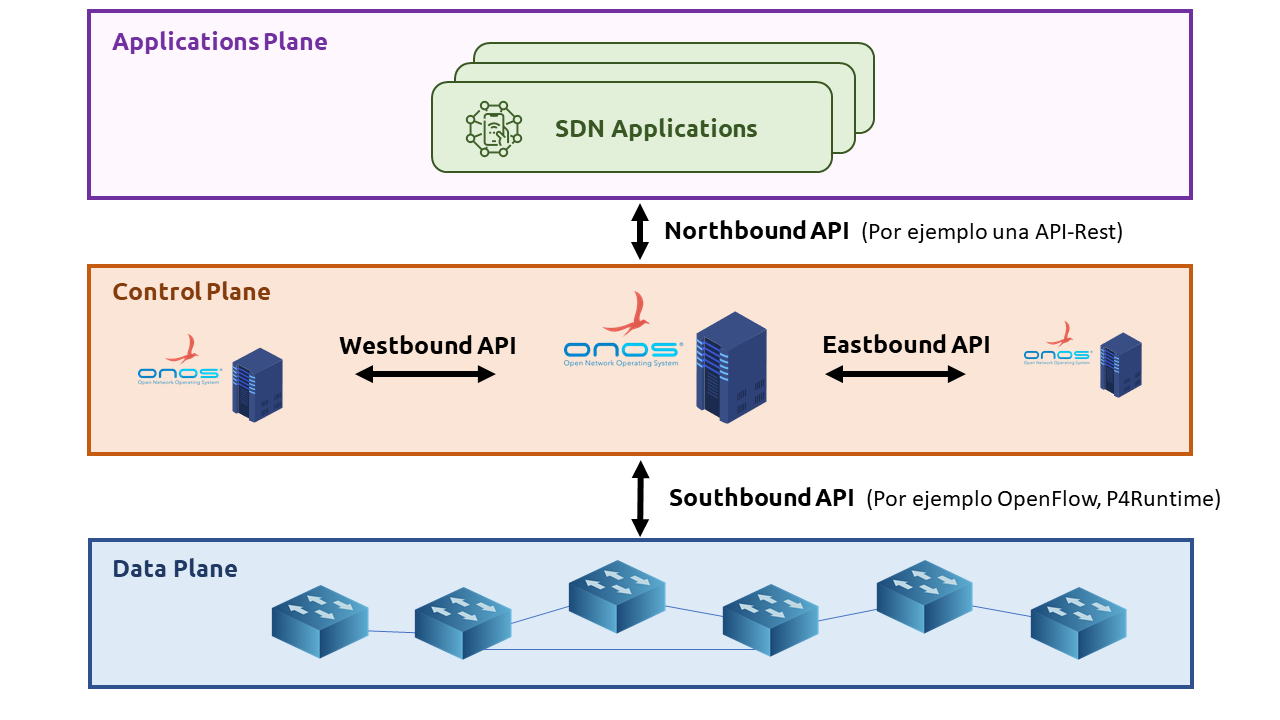
\includegraphics[width=14.5cm]{archivos/img/teoria/sdn_arch.png}
    \caption{Arquitectura básica \glsentryshort{sdn}}
    \label{fig:sdnBasicArch}
\end{figure}

\subsection{OpenFlow}

Existen varios protocolos para el control de los elementos de red desde el controlador, pero el más utilizado es Openflow. OpenFlow es un protocolo de la interfaz \textit{Southbound} que comunica los controladores \gls{sdn} con los elementos de red para configurar el estado de reenvío de estos últimos. La especificación de este protocolo se encuentra recogida por la \gls{onf}\footnote{\url{https://www.opennetworking.org/software-defined-standards/specifications/}}, contando con numerosas versiones siendo la última la versión \texttt{1.5.1} del 2015. \\
\par

El elemento clave de OpenFlow es el flujo (\textit{flow}), los cuales se conforman de paquetes que ha sido clasificados en función de reglas. Dichas reglas se encuentran en las tablas de flujo (\textit{flow table}) y  suelen estar relacionadas con los puertos de entrada o valores de cabecera típicos. Cuando estos criterios coinciden con los del paquete entrante se produce un \textbf{\textit{match}}.\\
\par
En el momento en que se produce un \textit{match}, el paquete en cuestión se verá sujeto a una serie de instrucciones asociadas a la regla con la que a hecho \textit{matching}. Estas instrucciones pueden ir desde, hacer una medición del paquete, aplicar una acción ó ir a otra tabla de flujo. De esta forma, con unas tablas de flujo completadas con unas reglas suministradas por el controlador \gls{sdn}, se conforma el estado de reenvío del switch en cuestión \cite{nadeau2013sdn}. 
